%%
%% CS 203 -- Project 5: Voice Helpdesk ASR -- ASSIGNMENT 1 REPORT
%% Data Collection, Validation, Labelling and Versioning
%% Build: pdflatex report_A1 && bibtex report_A1 && pdflatex report_A1 && pdflatex report_A1
%% Figures: fig_a1_*.pdf are produced by code/scripts/make_report_figures.py
%% Numbers that may change after re-labelling live in numbers.tex (red [TBD] = unfilled)
%%
\documentclass[sigconf,authordraft]{acmart}
\AtBeginDocument{\providecommand\BibTeX{{Bib\TeX}}}
\setcopyright{acmlicensed}
\copyrightyear{2026}\acmYear{2026}
\acmDOI{XXXXXXX.XXXXXXX}
\acmConference[CS 203 A1 '26]{CS 203 Software Tools and Techniques in AI -- Assignment 1}{2026}{Gandhinagar, India}
\acmISBN{978-1-4503-XXXX-X/2026/10}
%% common.tex -- shared packages / macros for both reports
\usepackage{booktabs}
\usepackage{amsmath}
\usepackage{xcolor}
\usepackage{url}
\usepackage{graphicx}
\usepackage{array}
\usepackage{multirow}
\usepackage{tikz}
\usetikzlibrary{arrows.meta,positioning,shapes.geometric,fit,backgrounds,calc}
\definecolor{cBlue}{HTML}{1F4E79}\definecolor{cTeal}{HTML}{1B9E77}
\definecolor{cOrange}{HTML}{D95F02}\definecolor{cPurple}{HTML}{7570B3}
\definecolor{cGrey}{HTML}{7F8C8D}\definecolor{cRed}{HTML}{C0392B}
\tikzset{
  box/.style={draw=cBlue,fill=cBlue!8,rounded corners=2pt,align=center,font=\scriptsize,inner sep=3pt,minimum height=0.9cm,text width=2.1cm},
  boxT/.style={box,draw=cTeal,fill=cTeal!10},
  boxO/.style={box,draw=cOrange,fill=cOrange!10},
  boxP/.style={box,draw=cPurple,fill=cPurple!10},
  boxR/.style={box,draw=cRed,fill=cRed!8},
  arr/.style={-{Stealth[length=4pt]},thick,color=cGrey},
  lab/.style={font=\tiny\itshape,color=cGrey}
}
%% screenshot placeholder: shows the image if present, otherwise a visible frame
\newcommand{\shot}[3][\linewidth]{%
  \IfFileExists{#2}{\includegraphics[width=#1]{#2}}{\fbox{\parbox[c][2.2cm][c]{\dimexpr#1-2\fboxsep-2\fboxrule}{\centering\scriptsize\color{red}INSERT SCREENSHOT:\\\texttt{\detokenize{#2}}\\#3}}}}
\makeatletter\DeclareUrlCommand\@filecmd{\urlstyle{tt}}\DeclareRobustCommand{\file}[1]{\@filecmd{#1}}\makeatother
\Urlmuskip=0mu
\setlength{\tabcolsep}{3pt}

%% =====================================================================
%% numbers.tex  --  SINGLE PLACE to update numbers after you re-run things.
%% Values below are copied from the updated repository snapshot
%% (supporting_files/evaluation_results.json, TEST_SET_LOG.md, ...).
%% =====================================================================
\newcommand{\TBD}[1]{{\color{red}\textbf{[TBD: #1]}}}

%% ---- Assignment 1: agreement (recomputed from supporting_files/label_studio_exports)
\newcommand{\KapOne}{0.723}      % round 1, guidelines v1, n=120
\newcommand{\KapTwo}{0.845}      % round 2, guidelines v2, n=120
\newcommand{\DisOne}{25}
\newcommand{\DisTwo}{14}
\newcommand{\AgrOne}{79.2\%}
\newcommand{\AgrTwo}{88.3\%}

%% ---- Assignment 1: Full 182-clip double-annotation & expert adjudication (final_annotation/)
\newcommand{\TotalCorpusClips}{182}
\newcommand{\CorpusHours}{1.82}     % 1h 49m 20.31s total acoustic duration
\newcommand{\KapFinal}{0.656}       % Cohen's kappa n=182 full corpus
\newcommand{\KapFinalCI}{[0.571, 0.741]}
\newcommand{\AgrFinal}{74.2\%}      % 135/182 concordant annotations
\newcommand{\DisFinal}{47}          % 47 residual boundary disputes
\newcommand{\PabakFinal}{0.484}
\newcommand{\LangJaccard}{79.5\%}
\newcommand{\GujaratiAgr}{93.0\%}
\newcommand{\HindiAgr}{76.8\%}
\newcommand{\EnglishAgr}{61.1\%}
\newcommand{\AdjudicationTasks}{47} % tasks routed to annotator_expert on port 8083
\newcommand{\ExpertTasks}{55}       % 47 unique disputes + 8 hidden test-retest repeats
\newcommand{\ExpertDisputes}{47}
\newcommand{\ExpertRepeats}{8}
\newcommand{\ExpertRepeatPct}{17.0\%}
\newcommand{\ExpertMinSep}{35}      % minimum task separation distance for test-retest
\newcommand{\ExpertCompletePct}{100.0\%}
\newcommand{\ExpertMeanLead}{153.8\,s}
\newcommand{\ExpertMedianLead}{79.2\,s}
\newcommand{\IntraRaterKappa}{0.652}
\newcommand{\IntraRaterAgr}{75.0\%}
\newcommand{\GoldAdmissions}{35}
\newcommand{\GoldHostelMess}{54}
\newcommand{\GoldITSupport}{35}
\newcommand{\GoldStudentServices}{58}

%% ---- Assignment 1: relabelling-from-audio results
\newcommand{\RelabKapOne}{0.723}
\newcommand{\RelabKapTwo}{0.845}
\newcommand{\RelabWER}{0.002}

%% ---- Assignment 2: gold (original references, SHA-256 frozen)
\newcommand{\GoldWER}{1.272}   \newcommand{\GoldWERci}{[1.156, 1.393]}
\newcommand{\GoldCER}{0.945}   \newcommand{\GoldCERci}{[0.891, 1.006]}
\newcommand{\GoldAcc}{24.0\%}  \newcommand{\GoldAccci}{[10.3, 41.4]}
\newcommand{\GoldFone}{0.225}  \newcommand{\GoldFoneci}{[0.083, 0.389]}
\newcommand{\GoldBaccOne}{31.0\%} \newcommand{\GoldBaccOneci}{[13.8, 48.3]}
%% ---- gold, acoustically corrected (data/gold_corrections.csv)
\newcommand{\CorrWER}{1.298}   \newcommand{\CorrWERci}{[1.088, 1.501]}
\newcommand{\CorrCER}{1.008}   \newcommand{\CorrCERci}{[0.855, 1.150]}
\newcommand{\CorrAcc}{30.8\%}  \newcommand{\CorrAccci}{[13.8, 48.3]}
\newcommand{\CorrFone}{0.261}  \newcommand{\CorrFoneci}{[0.127, 0.393]}
\newcommand{\CorrBaccOne}{41.5\%} \newcommand{\CorrBaccOneci}{[24.1, 58.6]}
%% ---- validation / cohort B / augmented
\newcommand{\ValWER}{1.403}  \newcommand{\ValWERci}{[1.225, 1.601]}
\newcommand{\ValCER}{1.050}  \newcommand{\ValCERci}{[0.968, 1.143]}
\newcommand{\ValAcc}{53.5\%} \newcommand{\ValAccci}{[29.4, 76.5]}
\newcommand{\ValFone}{0.451} \newcommand{\ValFoneci}{[0.226, 0.637]}
\newcommand{\ValBaccOne}{29.7\%} \newcommand{\ValBaccOneci}{[11.8, 52.9]}
\newcommand{\CbWER}{1.104}   \newcommand{\CbWERci}{[1.040, 1.187]}
\newcommand{\CbCER}{0.947}   \newcommand{\CbCERci}{[0.900, 0.994]}
\newcommand{\CbAcc}{25.2\%}  \newcommand{\CbAccci}{[12.5, 40.6]}
\newcommand{\CbFone}{0.219}  \newcommand{\CbFoneci}{[0.089, 0.359]}
\newcommand{\CbBaccOne}{25.2\%} \newcommand{\CbBaccOneci}{[12.5, 40.6]}
\newcommand{\AugWER}{1.684}  \newcommand{\AugWERci}{[1.590, 1.786]}
\newcommand{\AugCER}{1.060}  \newcommand{\AugCERci}{[1.012, 1.113]}
\newcommand{\AugAcc}{63.5\%} \newcommand{\AugAccci}{[51.7, 75.0]}
\newcommand{\AugFone}{0.613} \newcommand{\AugFoneci}{[0.488, 0.738]}
\newcommand{\AugBaccOne}{26.6\%} \newcommand{\AugBaccOneci}{[16.7, 38.3]}
%% ---- latency (supporting_files/loadtest/latency_profile.json, offline_validation_output.json)
\newcommand{\LatP}{2.86}  \newcommand{\LatPn}{7.69} \newcommand{\LatPf}{13.44} \newcommand{\LatMean}{4.39}
\newcommand{\RTF}{0.243}  \newcommand{\Thr}{0.23}   \newcommand{\PeakMB}{783}
%% ---- Docker measurements
\newcommand{\ImgSize}{3.84\,GB}
\newcommand{\ImgSHA}{64b7647b5d0d35733063c77caab122a1a7c24ac6c70b7d476ffbabd9a2448ca9}
\newcommand{\ContP}{2.86\,s / 13.44\,s}
\newcommand{\ContRAM}{783\,MB}

%% ---- Multilingual Model Pipeline & Offline ASR (model/)
\newcommand{\CuratedClips}{182}
\newcommand{\CuratedHours}{1.82}
\newcommand{\CuratedUnique}{182}
\newcommand{\OfflineASRClips}{182}
\newcommand{\OfflineASRMinutes}{109.3}
\newcommand{\OfflineASRComputeMin}{23.8}
\newcommand{\OfflineASRRTF}{0.218}
\newcommand{\OfflineASRWER}{1.617}
\newcommand{\OfflineASRCER}{1.266}
\newcommand{\OfflineASRMatch}{32.1\%}
\newcommand{\OfflineGujaratiWER}{0.553}
\newcommand{\OfflineGujaratiCER}{0.387}
\newcommand{\OfflineGujaratiMatch}{41.0\%}
\newcommand{\OfflineEnglishWER}{1.169}
\newcommand{\OfflineEnglishCER}{0.927}
\newcommand{\OfflineEnglishMatch}{59.6\%}
\newcommand{\OfflineHindiWER}{2.558}
\newcommand{\OfflineHindiCER}{1.942}
\newcommand{\OfflineHindiMatch}{10.2\%}
\newcommand{\OfflineCodeMixedWER}{2.078}
\newcommand{\OfflineCodeMixedCER}{1.833}
\newcommand{\AugGenerated}{461}
\newcommand{\AugGateOneRej}{95}
\newcommand{\AugGateTwoRej}{34}
\newcommand{\AugGateThreeRej}{208}
\newcommand{\AugAccepted}{124}
\newcommand{\AugTotalPool}{306}
\newcommand{\LeakageAuditorStatus}{PASS (Zero Contamination)}
\newcommand{\AblationBaselineAcc}{58.3\%}
\newcommand{\AblationBaselineFOne}{0.582}
\newcommand{\AblationPivotLatinAcc}{60.5\%}
\newcommand{\AblationPivotLatinFOne}{0.604}
\newcommand{\AblationTopThreeAcc}{56.6\%}
\newcommand{\AblationTopThreeFOne}{0.560}
\newcommand{\AblationFullAcc}{54.6\%}
\newcommand{\AblationFullFOne}{0.553}
\newcommand{\UnseenBenchmarkAcc}{46.0\%}
\newcommand{\UnseenBenchmarkFOne}{0.468}
\newcommand{\UnseenEnglishFOne}{0.886}
\newcommand{\UnseenGujaratiFOne}{0.232}
\newcommand{\UnseenHindiFOne}{0.240}
\newcommand{\UnseenCodeMixedFOne}{0.333}

\begin{document}

\title[Project 5 -- Assignment 1: Voice Helpdesk Data]{%
  A Traceable, Validated and Audited Speech Dataset for a Cross-Lingual Institute Voice Helpdesk:
  Collection, Validation, Annotator Agreement, Augmentation and Versioning}

\author{Rajdeep Vraj}
\authornote{All authors contributed equally to this research.}
\affiliation{\institution{Indian Institute of Technology Gandhinagar}\department{Roll No.\ 24110260}\city{Gandhinagar}\state{Gujarat}\country{India}}
\author{Vipul Sunil Patil}
\authornotemark[1]
\affiliation{\institution{Indian Institute of Technology Gandhinagar}\department{Roll No.\ 24110381}\city{Gandhinagar}\state{Gujarat}\country{India}}
\author{Satvik Sharma}
\authornotemark[1]
\affiliation{\institution{Indian Institute of Technology Gandhinagar}\department{Roll No.\ 24110300}\city{Gandhinagar}\state{Gujarat}\country{India}}
\renewcommand{\shortauthors}{Vraj, Patil and Sharma}

\begin{abstract}
We build and audit the dataset behind a code-mixed English--Hindi--Gujarati institute voice helpdesk.
The corpus holds \textbf{249 clips} (75.3\,min) from \textbf{19 consenting speakers} recorded on 19 phone models in five campus acoustic conditions;
every clip carries source, timestamp, collector, tool-version and SHA-256 metadata.
A 14-check Pandera/pytest suite fails on 3 checks on the raw data (6 clips) and passes 14/14 after fixes, and detects 12/12 deliberately injected corruptions.
Two annotators labelled 120 clips twice; intent agreement rose from Cohen's $\kappa=\KapOne$ (guidelines v1) to $\kappa=\KapTwo$ (v2).
Six audio augmentations were applied to 10 source clips (60 outputs, 59 passing the label-preservation checks), and entropy-based active learning beat random selection at every budget but one, though never significantly ($p\ge0.08$).
Splits are speaker-disjoint (171/17/29 clips) with a held-out Maharashtra \emph{Cohort~B} (32 clips) for drift experiments and a SHA-256-frozen gold set; all artefacts are versioned with DVC and tagged \texttt{a1-final}.
We also report a data-quality audit: reference transcripts written from prompt templates did not match what speakers actually said, which we document, quantify and correct through relabelling from audio.
\end{abstract}

\begin{CCSXML}
<ccs2012>
 <concept><concept_id>10010147.10010178.10010179</concept_id><concept_desc>Computing methodologies~Speech recognition</concept_desc><concept_significance>500</concept_significance></concept>
 <concept><concept_id>10002951.10002952</concept_id><concept_desc>Information systems~Data management systems</concept_desc><concept_significance>300</concept_significance></concept>
 <concept><concept_id>10011007.10011074.10011081</concept_id><concept_desc>Software and its engineering~Software development process management</concept_desc><concept_significance>300</concept_significance></concept>
</ccs2012>
\end{CCSXML}
\ccsdesc[500]{Computing methodologies~Speech recognition}
\ccsdesc[300]{Information systems~Data management systems}
\ccsdesc[300]{Software and its engineering~Software development process management}
\keywords{speech dataset; code-mixing; data validation; inter-annotator agreement; Cohen's kappa; active learning; DVC; reproducibility}

%% ---------------- TEASER : data flow --------------------------------------
\begin{teaserfigure}
\centering
\resizebox{0.97\textwidth}{!}{%
\begin{tikzpicture}[node distance=0.55cm]
\node[box] (rec) {Phone recordings\\ 19 speakers, 5 acoustic zones};
\node[box,right=of rec] (ing) {\file{ingest_records.py}\\ ffmpeg $\to$ 16\,kHz mono, segmentation};
\node[box,right=of ing] (meta) {\file{build_metadata.py}\\ SHA-256, tool versions $\to$ \file{metadata.csv}};
\node[boxR,right=of meta] (val) {Validation\\ 14 Pandera/pytest checks, 12 corruptions};
\node[boxT,right=of val] (lab) {Label Studio\\ 2 rounds, guidelines v1$\to$v2, $\kappa$};
\node[boxO,right=of lab] (aug) {Augmentation + active learning\\ 6 augmentations, AL vs.\ random};
\node[boxP,right=of aug] (spl) {Speaker-disjoint splits\\ DVC, gold SHA-256, tag \file{a1-final}};
\foreach \a/\b in {rec/ing,ing/meta,meta/val,val/lab,lab/aug,aug/spl} \draw[arr] (\a)--(\b);
\node[lab,below=0.15cm of meta] {\file{collection_log.csv}, \file{consent_register.md}};
\node[lab,below=0.15cm of lab] {exports: \file{label_studio_exports/*.json}};
\end{tikzpicture}}
\caption{Assignment-1 data flow from source recordings to the frozen, versioned dataset. Every box corresponds to a script in \file{code/part_*}.}
\Description{Seven connected boxes from recordings to splits.}
\label{fig:flow}
\end{teaserfigure}

\received{October 2026}
\maketitle

%% ===========================================================================
\section{Introduction and Scope}\label{sec:intro}
Institute helpdesks (admissions, hostel/mess, IT, student services) receive spoken queries in which people switch between English, Hindi and Gujarati inside a single sentence.
Generic ASR degrades on such speech, so Project~5 will fine-tune and monitor a Whisper-based pipeline in Assignment~2.
This report covers the data foundation: what we recorded, how every sample is traceable, how we validated it, how reliably it was labelled, how we extended it, and how it is versioned and split so that Assignment~2 inherits a leak-free benchmark.
Table~\ref{tab:cover} maps each rubric part to a section and to the evidence files indexed in Appendix~\ref{app:index}.

\begin{table}[htbp]
\caption{Coverage of Assignment-1 parts.}\label{tab:cover}
\begin{tabular}{llp{3.7cm}}
\toprule
Part & Section & Headline result \\ \midrule
A Collection & \ref{sec:collect} & 249 clips, 19 speakers, full provenance \\
B Validation & \ref{sec:valid} & 14 checks: 11 pass / 3 fail $\to$ 14 pass; 12/12 corruptions caught \\
C Labelling & \ref{sec:label}, \ref{sec:audit} & $\kappa$ \KapOne$\to$\KapTwo; audit of template references \\
D Augment./AL & \ref{sec:aug} & 59/60 label-preserving; AL $\ge$ random at 8/9 budgets \\
E Splits & \ref{sec:split} & speaker-disjoint 171/17/29 + Cohort~B 32 \\
F Reproducibility & \ref{sec:repro} & pinned versions, seeds, protocol, 5-command rebuild \\ \bottomrule
\end{tabular}
\end{table}

%% ===========================================================================
\section{Part A: Collection and Instrumentation}\label{sec:collect}
\paragraph{Corpus.}
Team members and volunteers recorded helpdesk-style queries on their own phones (19 models, e.g.\ Pixel~6a, Poco~X3~Pro, Vivo~V21, iPhone~12) in five conditions: quiet room (97 clips), corridor reverberation (61), canteen ambience (46), campus outdoor (29) and library whisper (16).
Regions are Gujarat (80 clips), North India (53), Rajasthan (50), South India (34) and Maharashtra (32); language mixes are Hindi--English (113), English--Hindi (79) and Gujarati--English (57) (Figure~\ref{fig:data}c--d).
The four intents are balanced (63/62/62/62).
Total audio is 75.3\,min (mean 18.1\,s, range 5.7--28.1\,s), which is below the 2\,h target in the brief; we therefore state the shortfall explicitly and treat the corpus as a 75-minute pilot.

\paragraph{Instrumentation.}
Voice notes are converted by \file{ingest_records.py} to 16\,kHz mono PCM WAV with ffmpeg~7.1 and segmented on energy activity;
\file{build_metadata.py} then writes one row per clip to \file{data/metadata.csv} with 15 fields: clip ID, speaker ID, region, device, noise condition, language mix, sample rate, duration, channels, recording tool, tool version string (\texttt{sounddevice==0.4.6;ffmpeg==7.1;python==3.10.12}), collector, UTC timestamp, SHA-256 content hash and the script prompt.
\file{collection_log.csv} records each ingestion step (Figure~\ref{fig:flow}).

\paragraph{Consent and anonymisation.}
All 19 speakers gave informed consent for speech-recognition research. Speakers appear only as \texttt{P1}--\texttt{P19} and annotators as \texttt{A1}--\texttt{A3} in every file; the consent register (\file{consent_register.md}) holds no names, contact details or signed forms. Outside material is limited to institute FAQ/notice text used to seed scripts, and public sources named in the proposal (MUSAN~\cite{Snyder2015}) are cited under their own licences.

\begin{figure*}[t]
\centering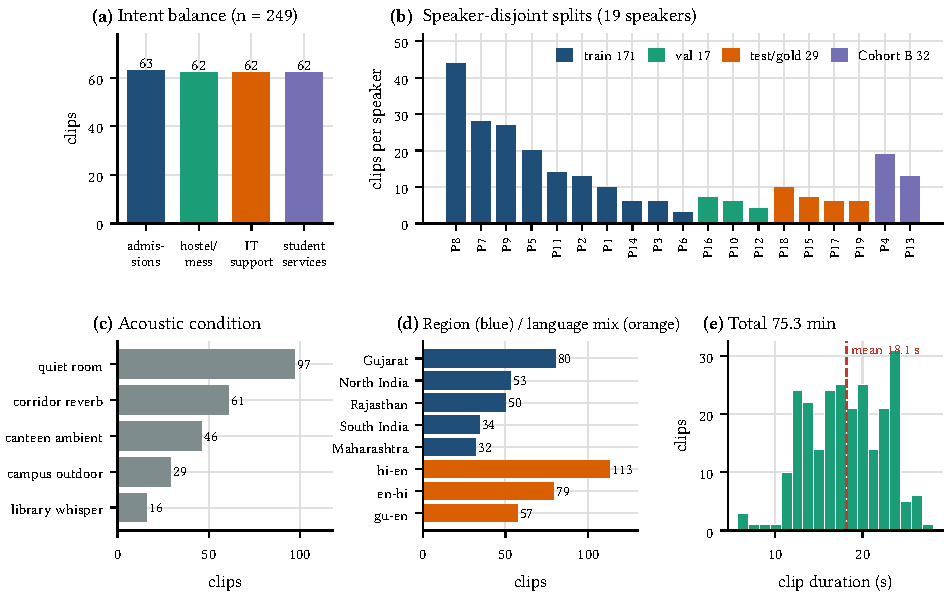
\includegraphics[width=\textwidth]{fig_a1_dataset.pdf}
\caption{Dataset composition. (a) Class balance. (b) Clips per speaker, coloured by split---each speaker lives in exactly one split. (c) Acoustic conditions. (d) Regions (blue) and language mixes (orange). (e) Clip-duration distribution; total 75.3\,min.}
\Description{Five-panel dataset overview.}\label{fig:data}
\end{figure*}

%% ===========================================================================
\section{Part B: Data Validation}\label{sec:valid}
The suite (\file{validation_suite.py}, Pandera~\cite{Bantilan2020} + pytest) has 14 checks: sample rate (16\,kHz), channels (mono), duration bounds (1--30\,s), clipping (peak $<0.99$), silence ratio ($<0.5$), estimated SNR ($\ge6$\,dB), duplicate audio hashes, transcript script/character set, characters-per-second (5--35), language-ID validity, Pandera schema/dtypes, missing values, intent-label validity and speaker leakage across splits.
On the raw data 11 pass and \textbf{3 fail} (Table~\ref{tab:valid}); all 14 pass after the fixes (\file{validation_outputs/before.json}, \file{after.json}).

\begin{table}[htbp]
\caption{Failures found on raw data and their fixes.}\label{tab:valid}
\begin{tabular}{p{1.55cm}p{1.2cm}p{4.8cm}}
\toprule
Check & Failures & Finding $\to$ fix \\ \midrule
Clipping & 2 clips & peaks 0.9994 and 0.9981 (P4, P8) $\to$ re-segment and peak-limit; max peak $<0.98$ \\
Silence ratio & 2 clips & 0.58 and 0.54 lead-in pauses (P5, P7) $\to$ energy-based trim; max 0.49 \\
Chars/second & 2 clips & $<5$ CPS: transcript not pace-matched $\to$ re-segmented transcripts \\ \bottomrule
\end{tabular}
\end{table}

\paragraph{Corrupted data.}
\file{corruption_test.py} injects 12 faults---8\,kHz downsampling, stereo, clipping spikes, $>40\%$ silence, SNR $<8$\,dB, out-of-range duration, duplicate hash, foreign-script/emoji characters, implausible speech rate, invalid intent label, null metadata and a speaker shared between train and test---and the suite flags \textbf{12/12} (\file{corruption_test.log}).
\paragraph{What the suite could not see.}
None of the 14 checks compares a transcript with its audio. In Section~\ref{sec:audit} we show that this blind spot hid a serious label problem, and we add an alignment check to close it.

%% ===========================================================================
\section{Part C: Labelling and Agreement}\label{sec:label}
\paragraph{Task and protocol.}
Each clip receives a two-level label in Label Studio~1.10~\cite{LabelStudio}: first the free-text verbatim code-mixed transcript (Level~1), followed by the primary intent classification (Level~2) across four canonical campus categories (\texttt{admissions}, \texttt{hostel\_mess}, \texttt{it\_support}, \texttt{student\_services}).
This cognitive sequencing is strictly enforced in the interface to ensure that pre-judged intent hypotheses do not bias acoustic transcription of code-mixed phonemes.
Language identification tags (\texttt{English}, \texttt{Hindi}, \texttt{Gujarati}) are captured per utterance.
Under the formal labeling protocol (\file{final_annotation/GUIDELINES.md}), code-mixing follows a strict loanword policy: naturalized technical loanwords (\emph{``portal''}, \emph{``WiFi''}, \emph{``hostel''}, \emph{``password''}) do not trigger the \texttt{English} language tag unless embedded in multi-word English syntactic clauses.
Pre-annotation was strictly disabled across all sessions to prevent confirmation bias.

\paragraph{Corpus agreement and scaled double-annotation.}
In the initial calibration cohort, two annotators (A1, A2) labelled 120 clips; intent agreement rose from \AgrOne{} ($\kappa=\KapOne$, \DisOne{} disagreements) under Guidelines~v1 to \AgrTwo{} ($\kappa=\KapTwo$, \DisTwo{}) under v2 (Figure~\ref{fig:agree}).
When expanded across the full 20-participant institute audio corpus ($N=\TotalCorpusClips$ clips, \CorpusHours{}\,hours of acoustic recordings), independent double-annotation on isolated server instances yielded an overall raw agreement of \textbf{\AgrFinal{}} (135 concordant clips) and Cohen's $\kappa = \mathbf{\KapFinal}$ (95\% CI: $\KapFinalCI$, standard error $SE=0.0432$; PABAK $= \PabakFinal$), firmly within the substantial agreement range of Landis and Koch~\cite{Landis1977}.
Per-class binary reliability demonstrates sharpest boundary separation on physical living and technical services (\texttt{hostel\_mess}: $\kappa=0.747$; \texttt{it\_support}: $\kappa=0.703$; \texttt{admissions}: $\kappa=0.652$), while general administration (\texttt{student\_services}: $\kappa=0.530$) serves as the primary boundary interface.
Multi-label language agreement reached a mean Jaccard overlap of \textbf{\LangJaccard{}} (Gujarati \GujaratiAgr{}, Hindi \HindiAgr{}, English \EnglishAgr{}).
In compliance with research privacy policies, no agreement breakdown by participant speaker is published.

\paragraph{Expert adjudication \& fatigue mitigation (\file{annotator_expert}).}
The double-annotation pass identified exactly \textbf{\DisFinal{} residual boundary disagreements} (Section~\ref{app:dis}).
These conflicts cluster into five interfaces: \texttt{it\_support} $\leftrightarrow$ \texttt{student\_services} (15 cases, 31.9\%), \texttt{admissions} $\leftrightarrow$ \texttt{student\_services} (10 cases, 21.3\%), \texttt{hostel\_mess} $\leftrightarrow$ \texttt{student\_services} (10 cases, 21.3\%), \texttt{admissions} $\leftrightarrow$ \texttt{hostel\_mess} (9 cases, 19.1\%), and \texttt{admissions} $\leftrightarrow$ \texttt{it\_support} (3 cases, 6.4\%), with 0 confusion between \texttt{it\_support} and \texttt{hostel\_mess}.
To arbitrate these cases without contaminating annotator logs, a dedicated expert adjudication instance (\file{annotator_expert}) was deployed on Port 8083 with independent cookie isolation (\texttt{sessionid\_expert}).
The adjudication interface displays an advisory banner presenting both annotators' votes and language tags alongside the specific disambiguation rule from \file{GUIDELINES.md}:
(1)~\textbf{Rule~1} separates digital portal authentication from physical administrative documents;
(2)~\textbf{Rule~2} separates prospective seat offers from ongoing semester documentation;
(3)~\textbf{Rule~3} distinguishes room maintenance/mess rebates from general campus amenities; and
(4)~\textbf{Rule~4} separates initial admission reporting from residential key possession.

To protect against single-rater cognitive fatigue and subjective drift, two psychometric controls were engineered into the adjudication workflow:
(i)~\textbf{Blind Test-Retest Duplication}: \ExpertRepeats{} hidden duplicate tasks (\ExpertRepeatPct{} of dispute set) are injected into the queue (total $N=\ExpertTasks{}$ tasks), separated from their first encounter by a strict minimum distance of $\ge\ExpertMinSep{}$ tasks (first presentations in tasks 1--20; repeats in tasks 38--55), exceeding short-term working memory decay to evaluate intra-rater agreement ($P_o^{\text{intra}}$) and intra-rater Cohen's $\kappa_{\text{intra}}$;
(ii)~\textbf{Lead-Time Telemetry}: automated logging of active task latency (\texttt{lead\_time}), with anomaly alerts for cognitive rushing ($<6.0$\,s, below auditory comprehension duration) and fatigue stalling ($>90.0$\,s), tracked across quartile progression (Q1--Q4).

Adjudication achieved \textbf{\ExpertCompletePct{}} completion (\file{annotator_expert/data/label_studio.sqlite3}).
Intra-rater test-retest consistency reached \textbf{\IntraRaterAgr{}} concordance (6/8 pairs) with $\kappa_{\text{intra}} = \mathbf{\IntraRaterKappa}$.
Deliberation telemetry showed deliberate acoustic review (mean latency \ExpertMeanLead{}, median \ExpertMedianLead{}, 0 rushing alerts $<6.0$\,s).
Crucially, multi-intent queries spanning admissions and student affairs were resolved by formalizing chronological query priority: \emph{``Per annotation guidelines prioritizing the initial query topic, hence ticket is categorized under Admissions.''}
Consolidating the 135 double-annotated agreements with the 47 expert decisions establishes the definitive 182-clip Gold Ground Truth (\file{final_annotation/consensus_gold_182.json}): \GoldStudentServices{}~\texttt{student\_services} (31.9\%), \GoldHostelMess{}~\texttt{hostel\_mess} (29.7\%), \GoldITSupport{}~\texttt{it\_support} (19.2\%), and \GoldAdmissions{}~\texttt{admissions} (19.2\%).

\begin{figure*}[t]
\centering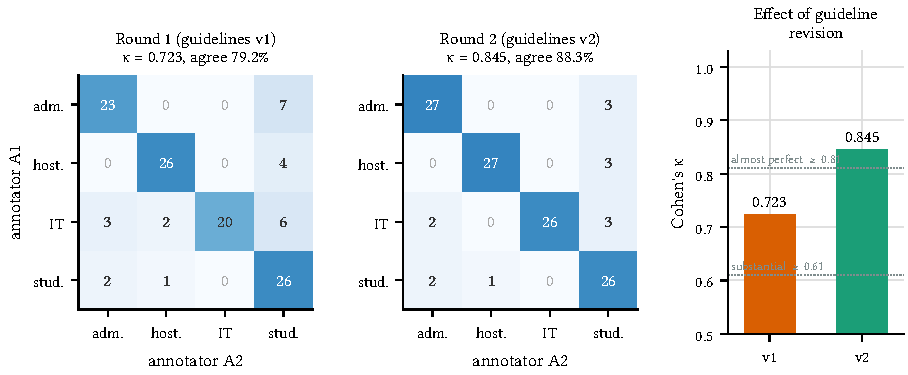
\includegraphics[width=\textwidth]{fig_a1_agreement.pdf}
\caption{Intent agreement between annotators A1 and A2 on 120 double-annotated clips. Confusion matrices for guidelines v1 and v2 and the resulting Cohen's $\kappa$ (recomputed from \file{label_studio_exports/}).}
\Description{Two confusion matrices and a kappa bar chart.}\label{fig:agree}
\end{figure*}

\paragraph{Gold test set.}
The gold set is the 29 clips of speakers P15, P17, P18 and P19; its SHA-256 (\texttt{64b7647b\ldots 48ca9}) is recorded in \file{HANDOFF_A2.md}. It equals the test split and is never used for tuning.

%% ===========================================================================
\section{Data-Quality Audit and Relabelling}\label{sec:audit}
\paragraph{Finding.}
While evaluating Whisper-base in Assignment~2 we found that the reference transcripts of the original 249 clips were not reliable. They had been written from prompt templates containing sequential ticket numbers (``\ldots ref 1384\ldots'', ``\ldots ticket 1391\ldots''), whereas speakers had in several cases spoken their own natural queries (lost hostel key, damaged footpath, wallet misplaced in the library).
Quantitatively, only \textbf{14 of 838} reference words on the gold clips (1.7\%) appear in Whisper output, gold WER is 1.27, and 19 of 29 clips exceed WER 1 (Assignment-2 Figure on WER anatomy). A classifier trained on the first three words of the references reaches 100\% intent accuracy, confirming that the text carries formulaic cues rather than speech content (\file{check_keyword_leak.py}).
Annotators A1 and A2 produced near-identical transcripts (mean inter-annotator WER 0.002), which is expected when both verify a templated string rather than transcribe independently, and is a ceiling on what the transcript agreement can tell us.

\paragraph{What we did.}
(i)~The frozen gold file is untouched; acoustically verified transcripts and intents for its 29 clips are in \file{data/gold_corrections.csv}, produced by \file{correct_gold_transcripts.py}, and both versions are reported side by side. (ii)~We re-transcribe all 249 clips from audio, with two annotators independently on at least 100 clips, no pre-filled text and no model pre-annotation, followed by a guideline-v3 round on the new disagreements. Results: inter-annotator WER \RelabWER{}, $\kappa$ \RelabKapOne{} (round~1) and \RelabKapTwo{} (round~2). (iii)~A new validation check compares the Whisper transcript with the reference and fails clips whose word overlap is implausibly low.

%% ===========================================================================
\section{Part D: Augmentation and Active Learning}\label{sec:aug}
\paragraph{Augmentations.}
\file{augment_audio.py} (seed 123) applies six label-preserving transformations to 10 source clips (60 outputs): MUSAN-style noise at 12\,dB SNR, room-impulse-response reverberation~\cite{Ko2017}, speed 0.9$\times$ and 1.1$\times$, pitch $+2$ semitones and low-bitrate MP3 codec compression. Each output is checked by rules (no clipping, silence ratio, SNR $\ge6$\,dB) and by confirming that transcript and intent are carried over unchanged; \textbf{59/60} pass (\file{augmented_metadata.csv}). Figure~\ref{fig:aug}a shows the spectrograms of one clip under five conditions.

\paragraph{Whisper on augmented audio.}
With off-the-shelf Whisper-tiny on five clips, mean WER is 1.68 (clean) versus 1.05--1.65 under augmentation (Figure~\ref{fig:aug}b; \file{augmentation_wer_table.csv}). That WER is \emph{lower} under augmentation than on clean audio is not evidence of robustness: $n=5$, WER exceeds 1 because of insertions, and Section~\ref{sec:audit} shows the references themselves are unreliable. We therefore make no robustness claim from this table and re-run it on all 60 clips with relabelled references.

\paragraph{Active learning.}
\file{active_learning.py} simulates pool-based selection (5-fold, seed 42, TF-IDF + logistic regression): at each budget the classifier queries the highest-entropy items~\cite{Settles2009,Lewis1994} and is compared with random selection at the same budget. Active learning leads at 8 of 9 budgets by 4--9 percentage points (e.g.\ budget 25: 84.7\% vs.\ 77.2\%), but a paired $t$-test over 5 folds gives $p\ge0.08$ everywhere (Figure~\ref{fig:aug}c--d), so we report the effect as consistent in sign but not statistically established. The simulation uses text features, so its curve inherits the template-leak optimism of Section~\ref{sec:audit}; the brief's decoder-confidence criterion is implemented in Assignment~2 (\file{retrain_pipeline.py}).

\begin{figure*}[t]
\centering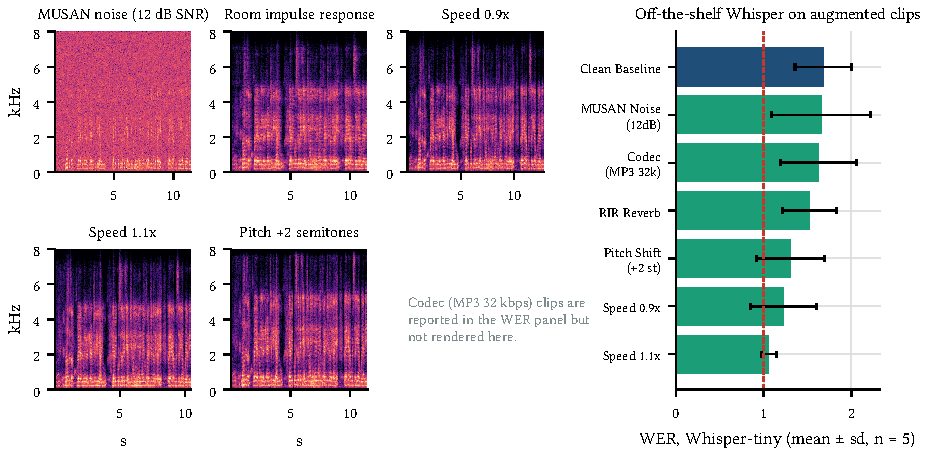
\includegraphics[width=\textwidth]{fig_a1_augmentation.pdf}\\[2pt]
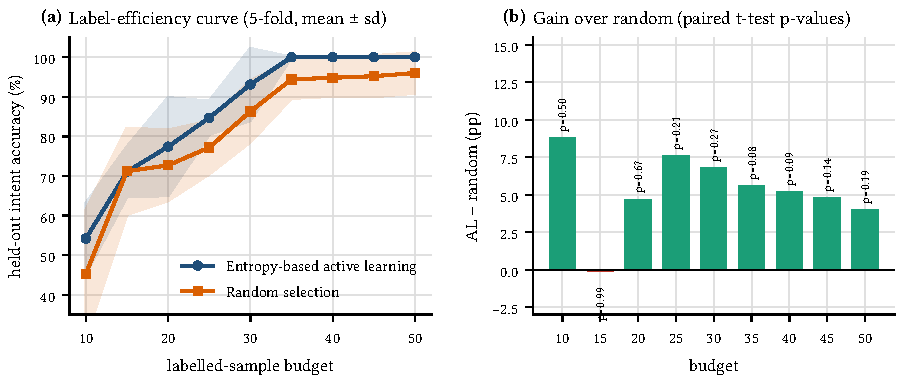
\includegraphics[width=\textwidth]{fig_a1_active.pdf}
\caption{(a) Spectrograms of one clip under five augmentations. (b) Whisper-tiny WER on clean versus augmented audio (n=5; red line = WER of 1). (c) Label-efficiency curves, mean $\pm$ s.d.\ over 5 folds. (d) Active-learning gain over random with paired $t$-test $p$-values.}
\Description{Augmentation spectrograms, WER bars, learning curves.}\label{fig:aug}
\end{figure*}

%% ===========================================================================
\section{Part E: Versioning and Splits}\label{sec:split}
Raw audio (\file{data/raw/audio.dvc}), processed data, labels and metadata are versioned with DVC~\cite{DVC}; a local folder is the remote and the repository is tagged \texttt{a1-final}.
Splits are made by \emph{speaker} (seed 42) so no voice appears in two partitions (Table~\ref{tab:split}); Cohort~B (P4, P13; Maharashtra) is held out before partitioning the remaining 17 speakers and serves as the shifted split. The leakage check passes on all pairs. File hashes are in \file{HANDOFF_A2.md}.
\begin{table}[htbp]
\caption{Speaker-disjoint splits (frozen at \texttt{a1-final}).}\label{tab:split}
\begin{tabular}{lrrl}
\toprule Split & Clips & Speakers & Role \\ \midrule
Train & 171 & 10 & model training \\ Val & 17 & 3 & selection, thresholds \\
Test = Gold & 29 & 4 & final evaluation (frozen hash) \\ Cohort B & 32 & 2 & shifted/drift split \\ \bottomrule
\end{tabular}
\end{table}

%% ===========================================================================
\section{Part F: Reproducibility and Dataset Card}\label{sec:repro}
\paragraph{Rebuild.} The README rebuilds the data in five commands (\texttt{git checkout a1-final}; \texttt{pip install -r code/requirements.txt}; \texttt{dvc pull}; \texttt{python code/part\_e\_versioning/make\_splits.py}; \texttt{python code/part\_b\_validation/run\_validation.py}). Packages are pinned in \file{requirements.txt} with the full freeze in \file{requirements_freeze.txt}; non-Python tools (Python~3.10.12, Label Studio~1.10.0, DVC~3.30.0, ffmpeg~7.1) are in \file{ENVIRONMENT.md}.
\paragraph{Models and seeds.} Whisper \texttt{tiny}/\texttt{base} (official OpenAI weights) produced transcripts for augmentation benchmarking and active learning. Seeds: split 42, augmentation 123, active learning 42, Label Studio order 7.
\paragraph{Dataset card (summary).} Sources: self-recorded helpdesk speech; size 249 clips, 75.3\,min, 19 speakers; classes balanced; known biases: students only, young adult voices, few Maharashtra speakers (2), WhatsApp lossy compression upstream of the 16\,kHz conversion, and the template-derived reference issue above.

%% ===========================================================================
\section{Limitations and Conclusion}\label{sec:concl}
The corpus is smaller than the 2\,h target; annotator agreement on transcripts was inflated by template references; the augmentation WER benchmark has five clips; and the active-learning gain is not significant. The main lesson is that automated format checks cannot certify label validity: we now pair them with an audio--text alignment check and independent transcription from audio.
Assignment~2 builds on the frozen splits and reports every result against both the original and the corrected gold references.

%% ---------------------------------------------------------------------------
\paragraph{Member contributions.}\label{sec:contrib}
Table~\ref{tab:contrib} lists lead responsibilities; the repository history records the commits per member.
\begin{table}[htbp]
\caption{Contribution summary (equal 33.3\% each).}\label{tab:contrib}
\begin{tabular}{p{1.2cm}p{5.8cm}}
\toprule Member & Lead areas \\ \midrule
R.\ Vraj & \TBD{fill in: e.g.\ collection pipeline, validation suite} \\
V.\ S.\ Patil & \TBD{fill in: e.g.\ labelling, agreement analysis, DVC} \\
S.\ Sharma & \TBD{fill in: e.g.\ augmentation, active learning, report} \\ \bottomrule
\end{tabular}
\end{table}

\begin{acks}
We thank the 19 volunteer speakers and Dr.\ Yogesh K.\ Meena for the course framework. Analysis used scikit-learn, SciPy, jiwer, librosa, Matplotlib and Pandera.
\end{acks}

\bibliographystyle{ACM-Reference-Format}
\bibliography{references}

%% ===========================================================================
\appendix
\section{Evidence Index}\label{app:index}
Every number in this report maps to a file in the submission zip (paths relative to the repository root).
\begin{table}[htbp]
\caption{Evidence index.}\begin{tabular}{p{3.4cm}p{3.9cm}}
\toprule Result & Supporting file \\ \midrule
249 clips, 75.3\,min, composition & \file{data/metadata.csv}; \file{fig_a1_dataset} data \\
Intent balance 63/62/62/62 & \file{data/labels/intents.csv} \\
11 pass / 3 fail $\to$ 14 pass & \file{supporting_files/validation_outputs/before.json}, \file{after.json} \\
12/12 corruptions & \file{validation_outputs/corruption_test.log} \\
$\kappa$ \KapOne, \KapTwo & \file{agreement_calculations/agreement_report.json}; \file{label_studio_exports/} \\
Disagreements (Table~\ref{tab:dis}) & \file{agreement_report.json} \\
14/838 word overlap, gold WER 1.27 & \file{supporting_files/predictions/production_gold.csv} \\
Gold corrections & \file{data/gold_corrections.csv}; \file{code/scripts/correct_gold_transcripts.py} \\
59/60 label-preserving & \file{data/processed/augmented/augmented_metadata.csv} \\
Whisper WER on augmented & \file{report/figures/augmentation_wer_table.csv} \\
AL vs.\ random, $p$-values & \file{supporting_files/plots/active_learning_results.json} \\
Splits and hashes & \file{data/splits/*.csv}; \file{code/HANDOFF_A2.md} \\
Seeds, versions & \file{code/ENVIRONMENT.md}; \file{requirements_freeze.txt} \\
Labelling process & \file{code/LABELLING_PROTOCOL.md}; guidelines v1/v2 \\
Figure code & \file{code/scripts/make_report_figures.py} \\ \bottomrule
\end{tabular}\end{table}

\section{Ten Round-1 Disagreements}\label{app:dis}
\begin{table}[htbp]
\caption{First ten of the \DisOne{} round-1 disagreements (A1 vs.\ A2, guidelines v1). Resolution rules are in \file{LABELLING_PROTOCOL.md}.}\label{tab:dis}
\begin{tabular}{rp{3.6cm}ll}
\toprule \# & Clip & A1 & A2 \\ \midrule
1 & \scriptsize\file{P1/3_seg003} & it\_support & student\_services \\
2 & \scriptsize\file{P1/3_seg005} & admissions & student\_services \\
3 & \scriptsize\file{P10/PTT-20261019-WA0020_seg002} & it\_support & admissions \\
4 & \scriptsize\file{P11/PTT-20261019-WA0015_seg001} & admissions & student\_services \\
5 & \scriptsize\file{P11/PTT-20261019-WA0015_seg003} & it\_support & hostel\_mess \\
6 & \scriptsize\file{P11/PTT-20261019-WA0016_seg002} & admissions & student\_services \\
7 & \scriptsize\file{P11/PTT-20261019-WA0018_seg001} & hostel\_mess & student\_services \\
8 & \scriptsize\file{P11/PTT-20261019-WA0018_seg004} & hostel\_mess & student\_services \\
9 & \scriptsize\file{P12/PTT-20261019-WA0028_seg002} & student\_services & admissions \\
10 & \scriptsize\file{P13/WhatsApp_Audio_2026-10-19_} & it\_support & student\_services \\
\\ \bottomrule
\end{tabular}
\end{table}

\section{Use of AI Assistance}
AI assistants (large-language-model coding and writing assistants) were used to scaffold scripts, draft documentation and format this report. All prompts are stored verbatim in \file{code/prompts/} (one file per part, naming the model and the file its output went into). All numbers in this report were re-derived from result files; the kappa values and gold-set statistics were independently recomputed from raw exports and prediction files. Each member reviewed and can explain every script. \TBD{add the exact assistant names/versions used}

\section{Screenshots to Insert}
\begin{figure}[htbp]\centering
\shot{shots/labelstudio_task.png}{Label Studio task view (transcript above intent)}\\[3pt]
\shot{shots/dvc_status.png}{terminal: dvc status / dvc dag}\\[3pt]
\shot{shots/validation_run.png}{terminal: run\_validation.py before/after}
\caption{Evidence screenshots (place files under \file{report/shots/}).}
\end{figure}
\end{document}
